\section{Characterizing Mobile Traffic}
\label{sec:measurement-results}

One of the key advantages of \meddle is that it serves as 
an ideal vantage point for monitoring network traffic 
generated by mobile devices across devices, OSes and 
carries. In this section we highlight some of the key observations 
we can make using \meddle.
%\subsection{Dataset Description}
%\label{sec:dataset-description}
%
%- IRB based study from September 2012. 
%- Full packet capture
%- Currently serves 20 devices from 14 users, 8 Android, 12 iOS device,    
%  4 iPads, 7 iPhones, and 1 iPod Touch.
%  15 service providers spread across US and France.
%- 30.2 GB of Traffic Volume from November 1, 2012

\subsection{Descriptive Statistics}
\label{sec:initial-results}

Below, we use several descriptive statistics to 
summarize our dataset and provide context for the remainder 
of the section. We focus on the type of traffic being generated, 
how it varies per OS and how it varies over different access technologies.

\noindent\textbf{Comparing across OSes.}
A key advantage of our approach is that it allows passive network 
monitoring across multiple OSes. In contrast, studies that rely on a custom, modified 
OS can monitor only devices configured to run the specific OS.
Table~\ref{tab:summaryIOSAndroidTraffic} directly compares Android and iOS, 
focusing on the portion of traffic using several key protocols. 

We classify IP flows as either TCP, UDP, or other. We further classify TCP flows as either HTTP, SSL, or
other. The SSL flows include HTTPS, IMAP, and other services that rely
on SSL to secure the connection between the mobile client and the
remote server. TCP flows that are not classified
as either HTTP or SSL are classified as other.  


\begin{table}
\begin{center}
\begin{tabular}{|l|l|r|r|r|r|}
\hline
\multirow{2}{*}{\bf Protocol} & \multirow{2}{*}{\bf Service} & \multicolumn{2}{|c|}{\bf Android} & \multicolumn{2}{|c|}{\bf iOS} \tabularnewline
\cline{3-6}
           &           &  \textbf{Flows}  &  \textbf{Bytes}  &  \textbf{Flows}  &  \textbf{Bytes}  \tabularnewline
\hline
 TCP       &  HTTP     &  14.87  &  74.31  &  16.07  &  82.01  \tabularnewline
\hline
TCP       &  SSL      &  37.19  &  24.35  &  37.64  &  17.31  \tabularnewline
\hline
 UDP       &  -        &  40.52  &   0.98  &  42.34  &   0.49  \tabularnewline
\hline
 TCP       &  other    &   2.08  &   0.22  &   1.13  &   1.89  \tabularnewline
\hline
 Other     &  -        &   5.35  &   0.14  &   2.82  &   0.09  \tabularnewline
\hline
\multicolumn{2}{|c|}{\emph{total}} & 100.00 & 100.00 & 100.00 & 100.00 \tabularnewline
\hline
\end{tabular}
\end{center}
\caption{Percentage of flows and bytes from iOS and Android devices. \tbd{Verify total 100
    for final results} \emph{SSL is responsible for the majority of
    TCP flows from iOS and Android devices.}} 
\label{tab:summaryIOSAndroidTraffic}
\end{table}

First, we observe that DNS is responsible for more 93.5\% of
the UDP flows. The rest of the flows are due to services such as
Skype. 
%421310/449421 

Second, we observe that most TCP traffic
traffic is HTTP, in line with previous results. Third, the majority 
of bytes are transferred over unencrypted channels. This is mainly 
due to streaming video (\eg, Netflix and YouTube) over HTTP. 

Last, we find the majority 
of TCP flows are sent over SSL, and these fraction is nearly identical 
for Android and iOS. We believe this occurs across platforms because 
the majority of flows come from e-mail, messaging and social networking, 
all of which use secure channels regardless of the OS.  

On balance the number of bytes transferred per unit time in Android, 
and the number of flows, is larger than the same for iOS. We found that iOS 
devices generated about 11.7\,MB of traffic per hour while Android devices 
generated about 15.5\,MB/hr, and increase of 33\%. Further, Android devices 
contributed more flows (505 per hour vs. 363 per hour), an increase of 40\%. 
It is difficult to account for the impact of user behavior on device-generated 
traffic; that aside, one explanation is that Android devices generate more 
bytes and flows due to the relatively permissive API for running code in the 
background on Android. In contrast, iOS quickly kills processes that 
are in the background, preventing them from generating network 
traffic after only a few seconds of losing the foreground.

%        oper_sys        BytesPerHour    FlowsPerHour    ndevices        normBytesPerHour        normFlowsPerHour
%1       Android 108628724       3539.354        7       15518389        505.6219
%2       iOS     93433575        2908.240        8       11679197        363.5300



\begin{table}
\begin{center}
\begin{tabular}{|l|l|r|r|r|r|}
\hline
\multirow{2}{*}{\bf Protocol} & \multirow{2}{*}{\bf Service} & \multicolumn{2}{|c|}{\bf Wi-Fi} & \multicolumn{2}{|c|}{\bf Cellular} \tabularnewline
\cline{3-6}
           &           &  \textbf{Flows}  &  \textbf{Bytes}  &  \textbf{Flows}  &  \textbf{Bytes}  \tabularnewline
\hline
 TCP       &  HTTP     &  16.91  &  83.52  &  13.03  &  56.14  \tabularnewline
\hline
 TCP       &  SSL      &  38.18  &  15.83  &  36.14  &  41.42  \tabularnewline
\hline
UDP       &  -        &  41.43  &   0.49  &  41.56  &   1.67  \tabularnewline
\hline
TCP       &  other    &   1.38 &   0.16  &   1.95  &   0.4  \tabularnewline
\hline
Other     &  -        &   2.12  &  0.01  &   7.2  &   0.3  \tabularnewline
\hline
\multicolumn{2}{|c|}{\emph{total}} & 100.00 & 100.00 & 100.00 & 100.00 \tabularnewline
\hline
\end{tabular}
\end{center}
\caption{Percentage of flows and bytes using Wi-Fi and Cellular as access technology. \tbd{Verify total 100
    for final results} \emph{The share of SSL traffic over Cellular
    networks is larger than its share over Wi-Fi.}}  
\label{tab:summaryWifiCellularTraffic}
\end{table}


\noindent\textbf{Comparing across access technologies.} Another 
key advantage of \meddle is that it allows us to passively monitor traffic 
regardless of whether a device is on \wifi or cellular, without 
needing any OS modifications or imposing any constraints on 
user mobility. In contrast, studies relying on traffic seen over campus \wifi~\cite{chen:wifi} miss traffic 
over cellular connections; those from cellular providers~\cite{gerber:passivespeed} miss \wifi traffic. 
As a point of reference, we found that the portion of network traffic  
generated by devices were nearly equally split (60/40) between 
\wifi and cellular (respectively), motivating the need to monitor both.

In \fref{tab:summaryWifiCellularTraffic}, we summarize the network 
traffic generated by \meddle-enabled devices over \wifi and cellular.
The first key observation is that the portion of HTTP bytes sent over \wifi and cellular 
are significantly different. Upon further inspection, we found that Wi-Fi is the
preferred medium to transfer media content, which generates relatively large flows. 
Another key reason is that apps such as
Google Plus image backup on Android allow users to upload their
images only over Wi-Fi. In line with the difference in HTTP traffic ratios, we 
note that SSL traffic is the dominant type in cellular connections.

We note that the portion of ``other'' flows for cellular on Android is a relatively large 7.2\%. This corresponds 
to ICMP traffic and occurs because 
several users run \emph{Mobiperf}, an application that performs regular network-measurement 
tests suing ICMP, and the measurements occur only over cellular connections.

%SSL traffic is typically compressed - discussion on compression
%opportunities for HTTP over Cellular networks refer to section ... for
%more details. We can refer to this section to introduce
%compression.

\noindent\textbf{Enabling direct performance comparisons.} 
Historically, cellular performance has lagged significantly behind 
\wifi, mainly for capacity reasons. With the advent of LTE and the 
increased interference from dense \wifi deployments, we investigate whether 
this common knowledge remains valid. 

Previous work by Sommers et al.~\cite{sommers:cellwifi} studied 
this question using SpeedTest results from a metro area, but did not 
have sufficient location accuracy to directly compare performance over 
\wifi and cellular for the same device. When considering a broad geographic 
region in aggregate, they found better performance 
from \wifi in the vast majority of cases. 

To directly compare \wifi and cellular performance for the same device, 
we determine the maximum transfer rate per hour for each device, 
then focus on cases where there was a sample for \wifi and cellular in 
the same hour. We restrict our analysis to users that transferred more than 100\,MB of 
data in a single month. Figure~\ref{fig:datarates} depicts the median 
and quartiles of these peak rates. The graph shows that for many users 
\wifi is better than cellular. However, users 4, 6 and 7 
often have better peak transfer rates over cellular -- mainly due to 
adoption of LTE. For user 4, however, we see that \wifi performance is 
poor compared to other users, indicating that some users may see better 
connections over cellular connections even if they are using 3G or older 
technologies. This highlights opportunities for proposals such as 3G onloading~\cite{vr:3gol}.

\begin{figure}
\vspace{-2.5em}
\centering
        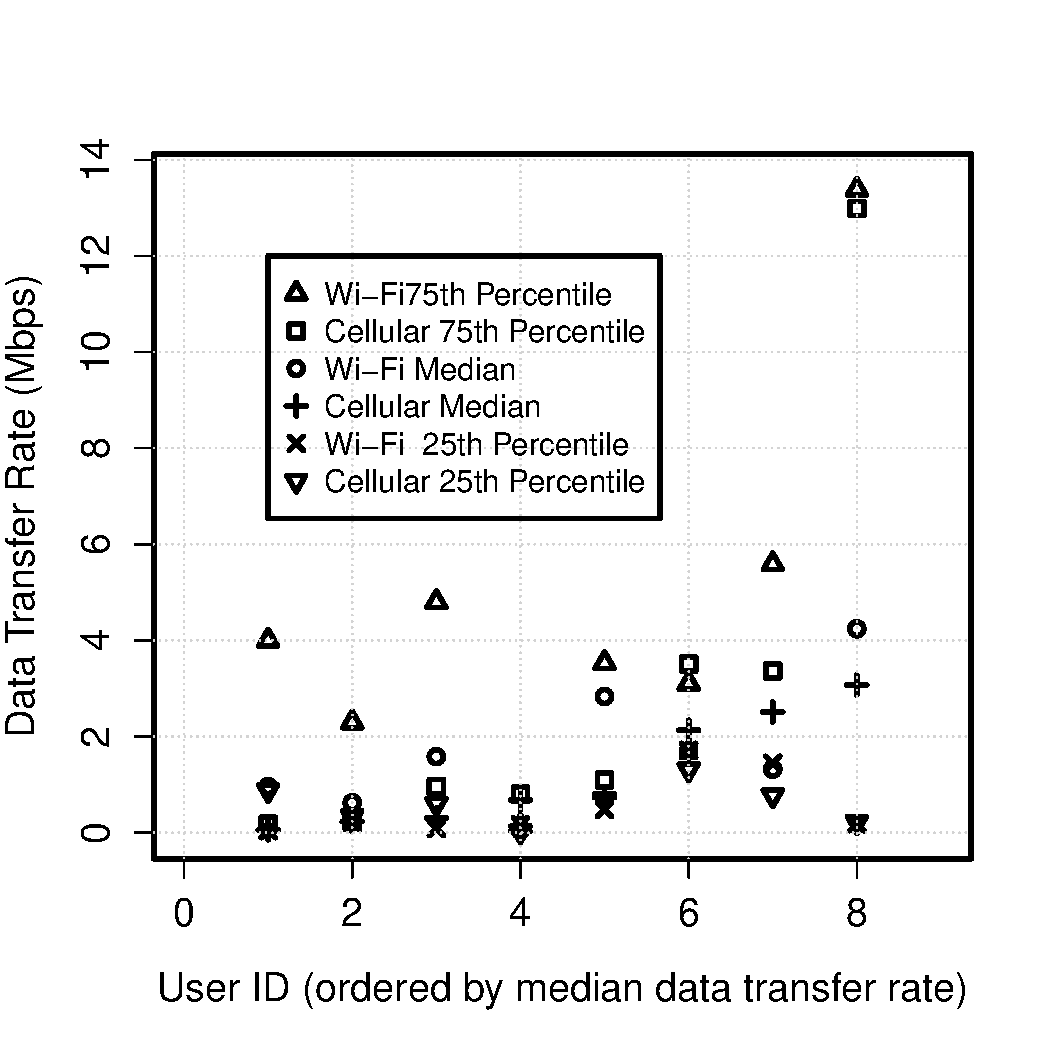
\includegraphics[width=\linewidth]{./plots/dataRate.pdf}
  \caption{Median and quartile peak transfer rates for users when on \wifi 
  compared to cellular. Many users see significantly better performance 
  from \wifi; however, users with LTE often receive better performance over 
  cellular than \wifi.}
  \label{fig:datarates}
  \vspace{\postfigspace}
\end{figure}

\subsection{Case Study: Device Specific Apps (iOS Push)}
\label{sec:case-study-ios}

In this section, we present the results of a detailed case study 
of iOS push. We focus on this application because it represents 
an OS-managed service on an operating system that received 
little research attention due to its closed-source nature. 

We set out to answer the following questions: (1) What is the 
empirical network impact of push notifications and does the 
measured activity coincide with published documentation?
(2) Using \meddle, is there any relevant data traffic that is 
not captured by the VPN tunnel? (3) What is the impact of 
a VPN connection on network behavior? (4) Can we use 
network traffic alone to infer the state of the device?

\noindent \textbf{iOS Push Under the Microscope.} 
The Apple Push Notification Service 
(APNS) implements push for iOS. The documentation for APNS provides limited details about 
the implementation, but does specify expected behavior (\eg, push 
connections are established over cellular connections even if 
\wifi is available). 

We explicitly verified all provided documentation and confirmed that 
all statements are true with the exception of the notification behavior 
with an iPad. The documentation states that the iPad will always 
remain associated with a \wifi AP, even if it is not plugged in. Our 
experience shows this is not the case on an iPad 2.

We now further investigate 
the behavior of iOS push over time for three characteristic users. Figure~\ref{fig:pushHourly} 
plots this in terms of the median number of push notifications received per 
user per hour. During the period, all users were in the same time zone.

\begin{figure}
\vspace{-2.5em}
\centering
        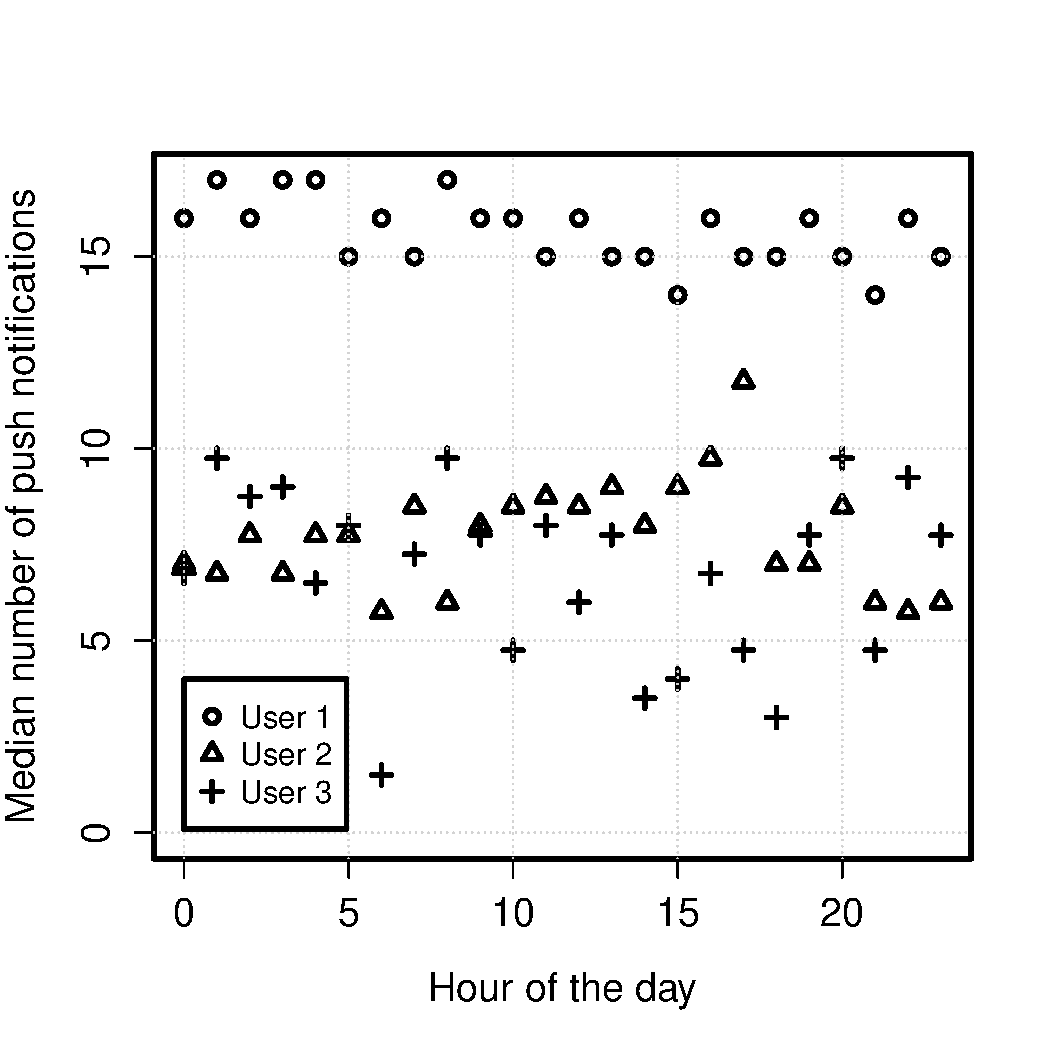
\includegraphics[width=\linewidth]{./plots/iosPushHourDistrib.pdf}
  \caption{Median number of push notifications seen per hour for three devices. 
  A significant number of updates occur at all hours, even during idle and ``do not disturb'' periods.}
  \label{fig:pushHourly}
  \vspace{\postfigspace}
\end{figure}

First, the figure shows that all three users see significant numbers of push 
notifications even in idle, overnight periods. It is unclear what the value of 
such traffic is. Second, we clearly see significant differences in the volume 
of traffic among users. User 1 has registered to receive push notifications 
from multiple apps, while Users 2 and 3 have not. Last, we note that even 
with iOS 6's ``do not disturb'' (DND) feature, push notifications continue to be 
sent during DND periods. Specifically, User 2 has enabled DND between 
midnight and 7am, but there is no noticeable change in APNS traffic.
In summary, we can use \meddle to help understand the network 
behavior of closed systems; further, we identify several opportunities 
where we believe the OS can reduce or eliminate push traffic (during idle periods).

% DRC: This contradicts results presented later.
%\tbd{Are we sure that devices are getting SMS notifications to connect to an apple server?}
%When a push notification is received, the iOS device connects to port
%5223 of a nearby Apple server. For each iOS device in our dataset, we
%logged the timestamp at which these connections were established. From
%this set of connections, we then selected the connections established
%between midnight and 6 am of the users local time. For each user, we
%computed the median of time interval between successive
%connections. We observe this median to be in the range of 190 seconds
%to 590 seconds. This time interval depends on the different apps for
%which the user has enabled notifications. 
%\tbd{Add figure}
%
%A user can disable notifications for specific time intervals on
%devices running iOS 6. In our dataset, three devices had notification
%disabled during different time intervals. During these time intervals
%we did not observe any traffic for notifications.

\noindent\textbf{Interaction between \meddle and the power management
  policy on iOS.}
In the remainder of this section, we perform controlled experiments 
to understand the interaction between \meddle's VPN connection and the power
management policy on iOS. In summary, we find that the impact of the VPN depends 
on the power state and network interfaces used (\wifi or cellular) on the
device -- but we show that the current power management policy on iOS
might adversely impact the energy consumption when the APNS is heavily used.
Further, we find that the changes in traffic patterns are relatively 
easy to identify, meaning \emph{we can use traffic from \meddle to infer 
when a device is plugged in and which access technologies are 
available}.

All the following experiments are performed on an \iphone 4 with iOS
6.0.1.  At the beginning of each experiment we close all applications
and restart the \iphone{}. The \iphone{} is connected in \wifi{} to a
controlled access point on which we perform a tcpdump on the \wifi{}
interface and monitor the \wifi{} association between the access point
and the \iphone{}. Each experiment lasts for around 1 hour. 

\begin{figure}
\centering
        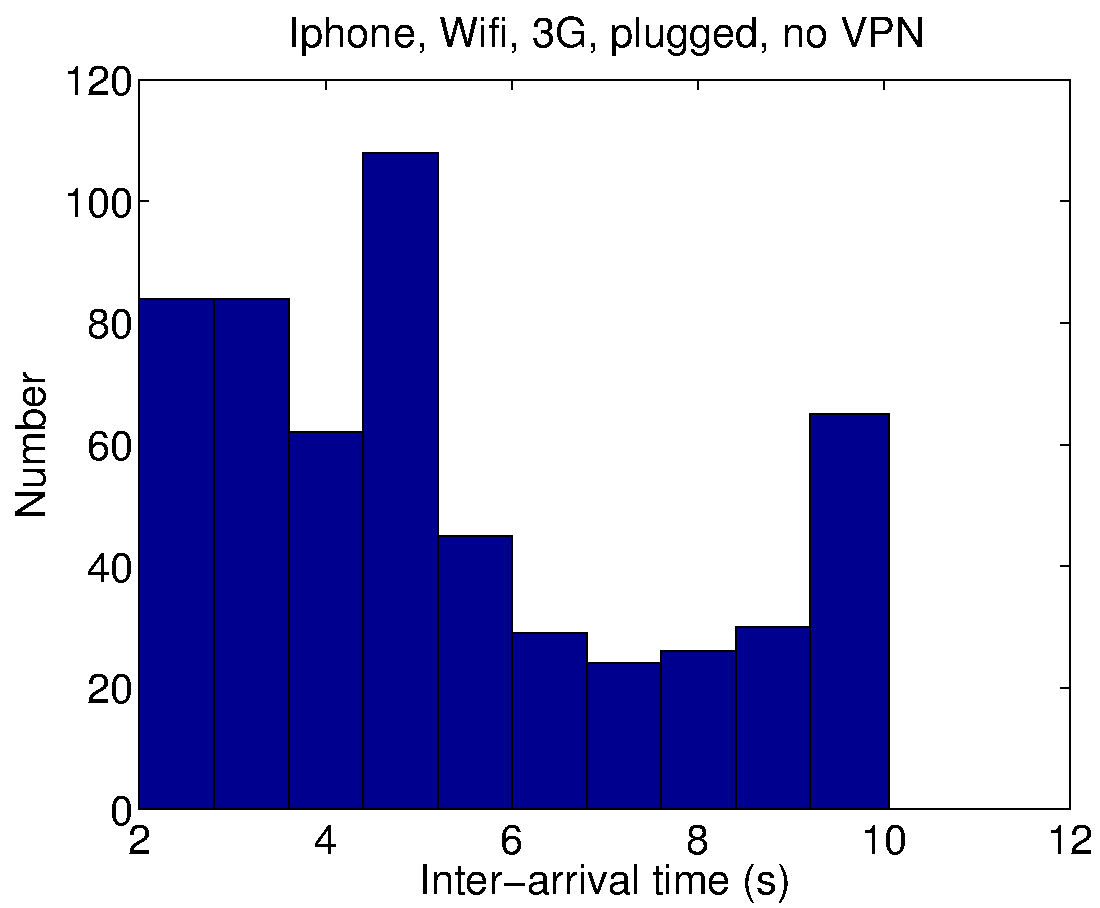
\includegraphics[width=0.8\linewidth]{../../code/pushNotification/Fig/bw_iphone_wifi_3g_plug_novpn_interTs.pdf}
  \caption{Distribution of the interarrival times of Ethernet frames
    for a one hour experiment with an idle \iphone{} plugged-in, with \wifi{} and cellular
    enabled, and no VPN enabled. For each bin of 1 second, we count
    the number of interarrivals in that bin.}
  \label{fig:push_w3p_interTs}
  \vspace{\postfigspace}
\end{figure}

%\begin{figure}
%\centering
%        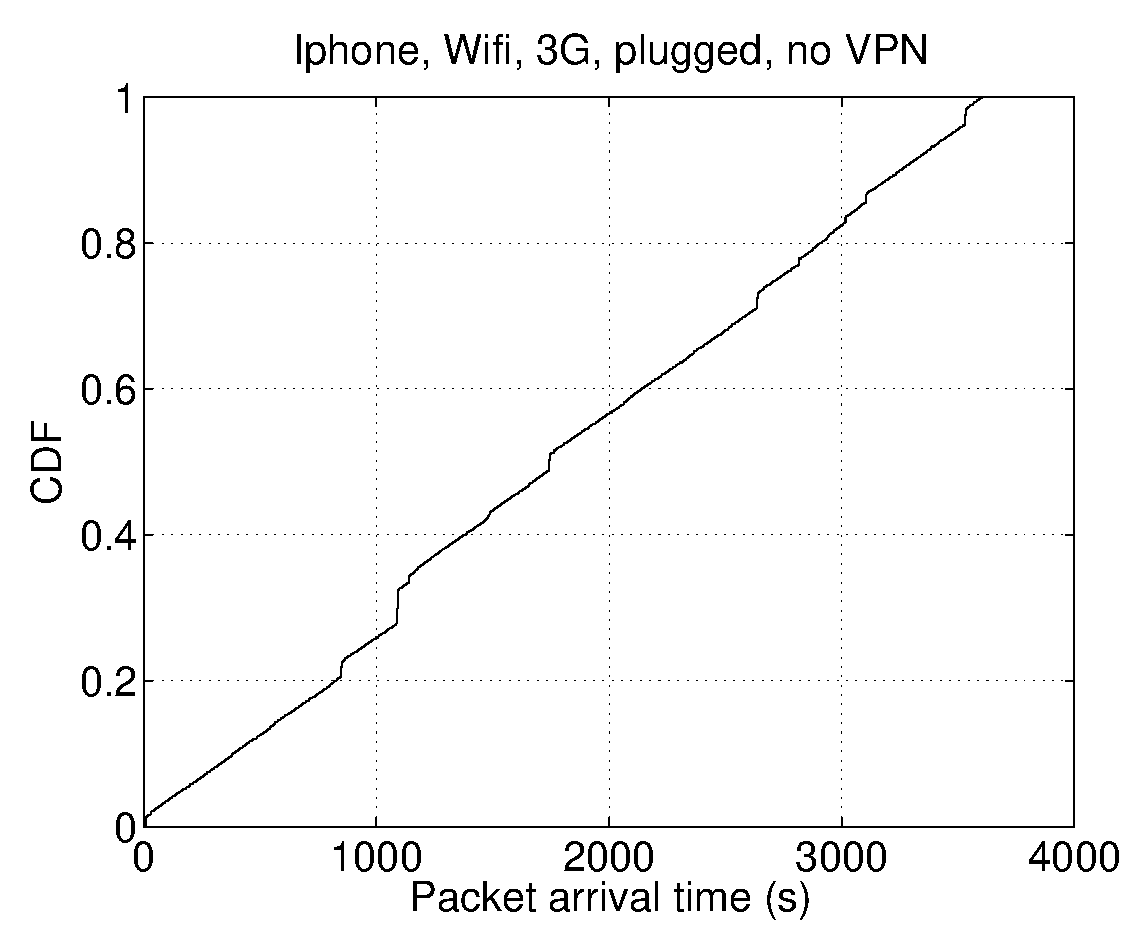
\includegraphics[width=0.8\linewidth]{../../code/pushNotification/Fig/bw_iphone_wifi_3g_plug_novpn_ts.eps}
%        \caption{Cumulative distribution of the Ethernet frames
%          arrival with time for a one hour experiment with an idle
%          \iphone{} plugged-in, with \wifi{} and 3G enabled, and no VPN
%          enabled.}
%  \label{fig:push_w3p_ts}
%\end{figure}

%\begin{figure}
%\centering
%        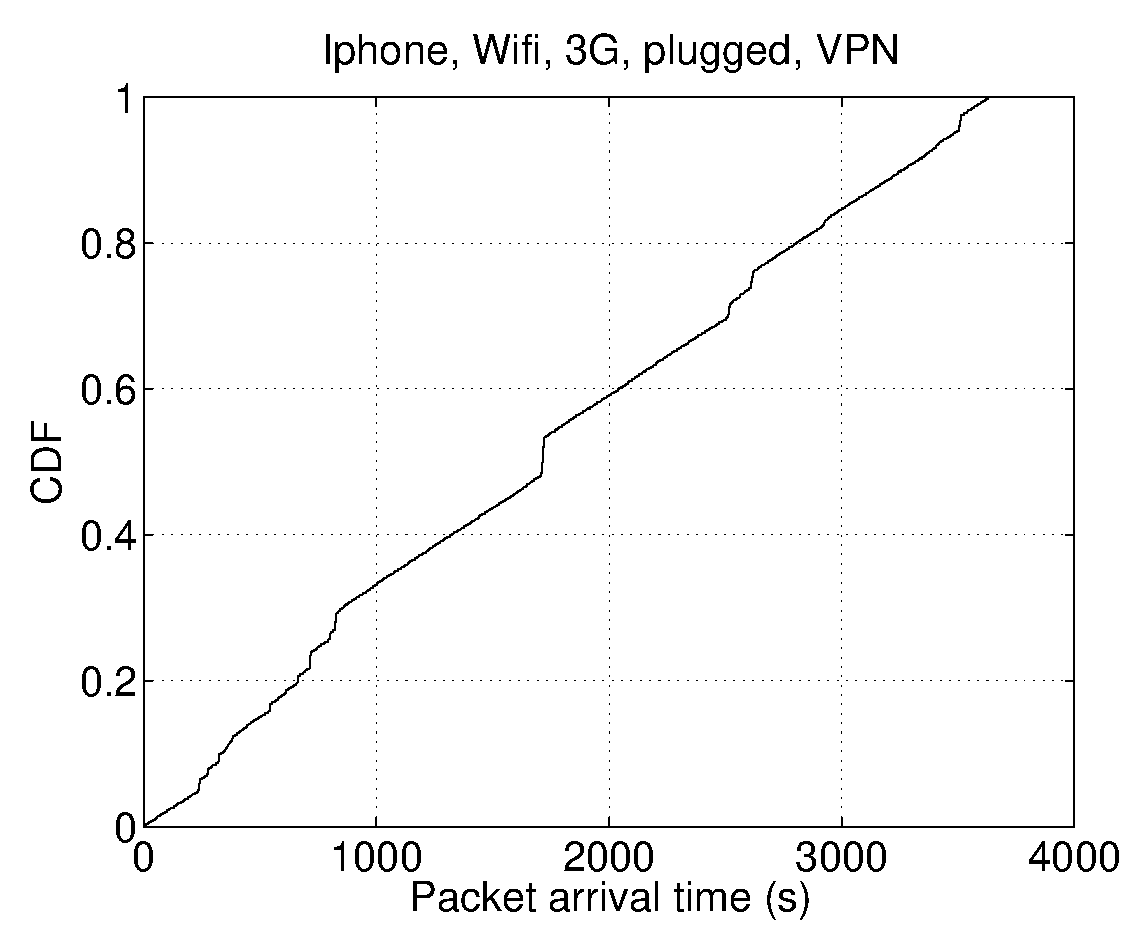
\includegraphics[width=0.8\linewidth]{../../code/pushNotification/Fig/bw_iphone_wifi_3g_plug_vpn_ts.eps}
%  \caption{Cumulative distribution of the Ethernet frames
%          arrival with time for a one hour experiment with an idle
%          \iphone{} plugged-in, with \wifi{} and 3G enabled, and VPN
%          enabled.}
%  \label{fig:push_w3pv_ts}
%\end{figure}

\noindent\emph{Behavior when plugged in.} When an \iphone{} is plugged-in, it always remains associated with the
\wifi{} access point if \wifi{} is enabled on the device. We performed
a first set of experiments to observe the traffic to and from an idle
\iphone{}. We see in Fig.~\ref{fig:push_w3p_interTs} and
Fig.~\ref{fig:push_w3pv_interTs} that the largest interarrival between
two frames is in the order of 10 seconds for both the VPN and no VPN
scenarios. We also observe no noticeable difference in the arrival of
frames with time for both scenarios. (The corresponding figures are 
omitted for space reasons.)
%(see Fig.~\ref{fig:push_w3pv_ts} and
%no VPN (see Fig.~\ref{fig:push_w3p_ts}) scenarios. 
\emph{Thus, it appears that the VPN connection has no noticeable
  impact on network traffic pattern when the device is plugged in.}


\begin{figure}[t]
\centering
        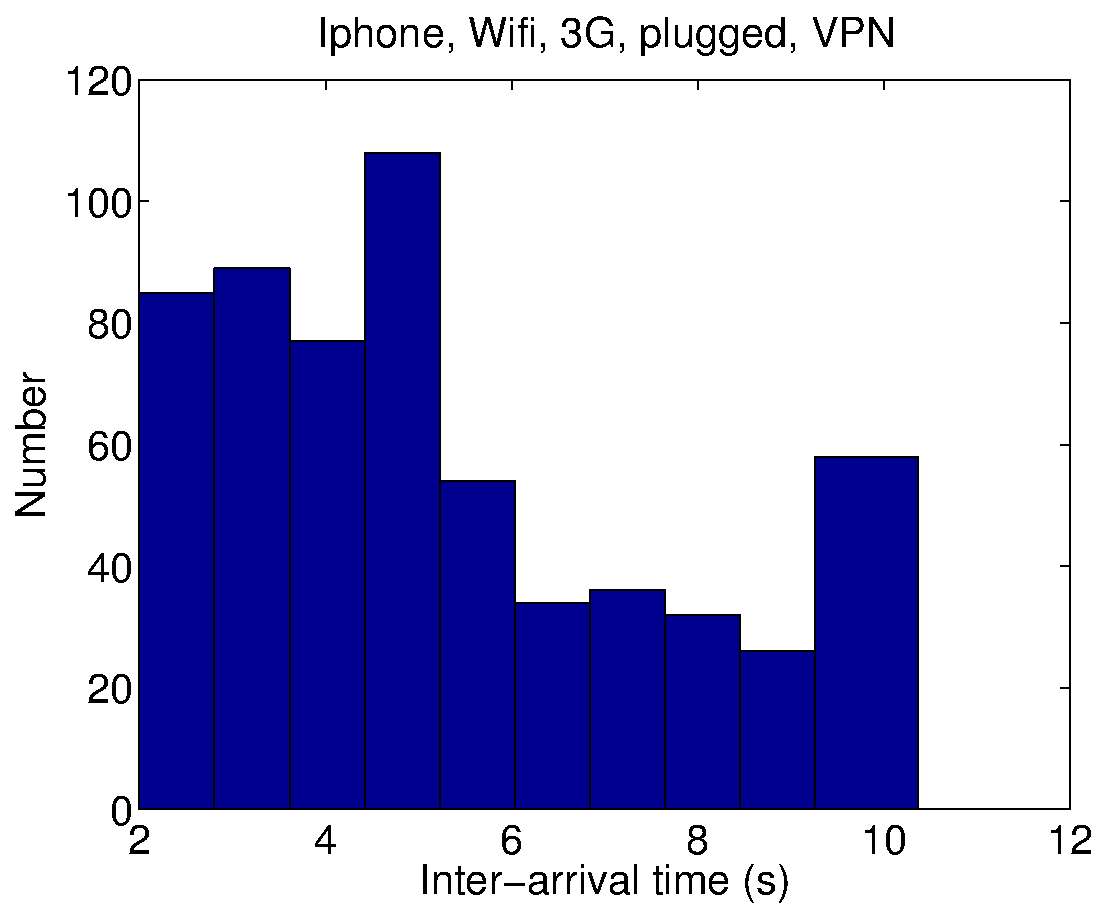
\includegraphics[width=0.8\linewidth]{../../code/pushNotification/Fig/bw_iphone_wifi_3g_plug_vpn_interTs.pdf}
  \caption{Distribution of the interarrival times of Ethernet frames
    for a one hour experiment with an idle \iphone{} plugged-in, with \wifi{} and cellular
    enabled, and VPN enabled. For each bin of 1 second, we count
    the number of interarrivals in that bin.}
  \label{fig:push_w3pv_interTs}
   \vspace{\postfigspace}
\end{figure}


%We don't claim this
%traffic to be typical, in particular, our access point is a Windows 7
%machine sending SSDP traffic to announce available services. Instead,
%we use it to understand in our experimental setup the background
%traffic.

%\begin{figure}
%\centering
%        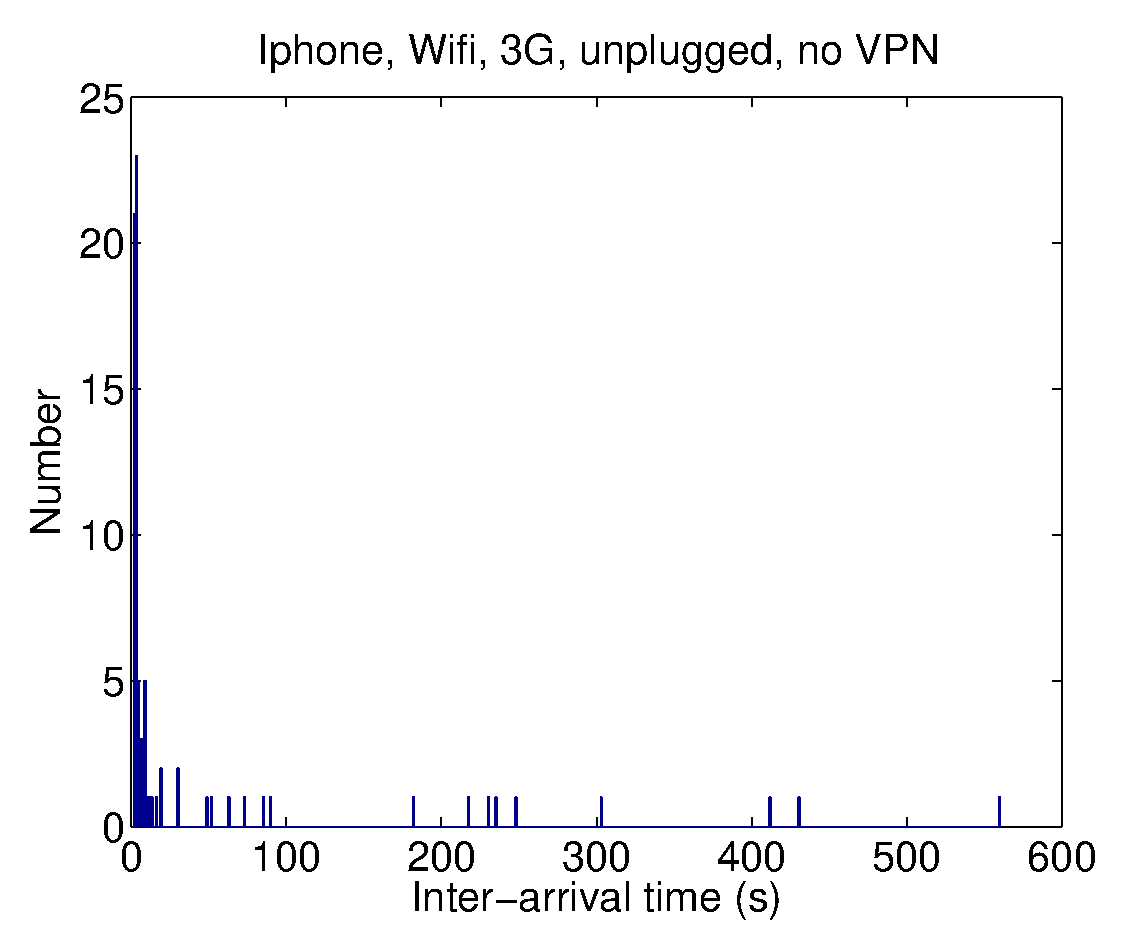
\includegraphics[width=0.8\linewidth]{../../code/pushNotification/Fig/bw_iphone_wifi_3g_unplug_novpn_interTs.eps}
%  \caption{Distribution of the interarrival times of Ethernet frames
%    for a one hour experiment with an idle \iphone{} unplugged, with \wifi{} and 3G
%    enabled, and no VPN enabled. For each bin of 1 second, we count
%    the number of interarrivals in that bin.}
%  \label{fig:push_w3_interTs}
%\end{figure}


\noindent\emph{Behavior when on battery.} 
In a second set of experiments, we consider a default \iphone{}
setting with cellular and \wifi{} enabled, and the \iphone{} unplugged. This
corresponds to a typical setting for a user on move.  We observed 
relatively large interarrival times for frames in this case (many on the order of 100s of 
seconds). These cases correspond to
periods during which the \wifi interface of the \iphone{} is not
associated to the access point for energy saving. 


%\begin{figure}
%\centering
%        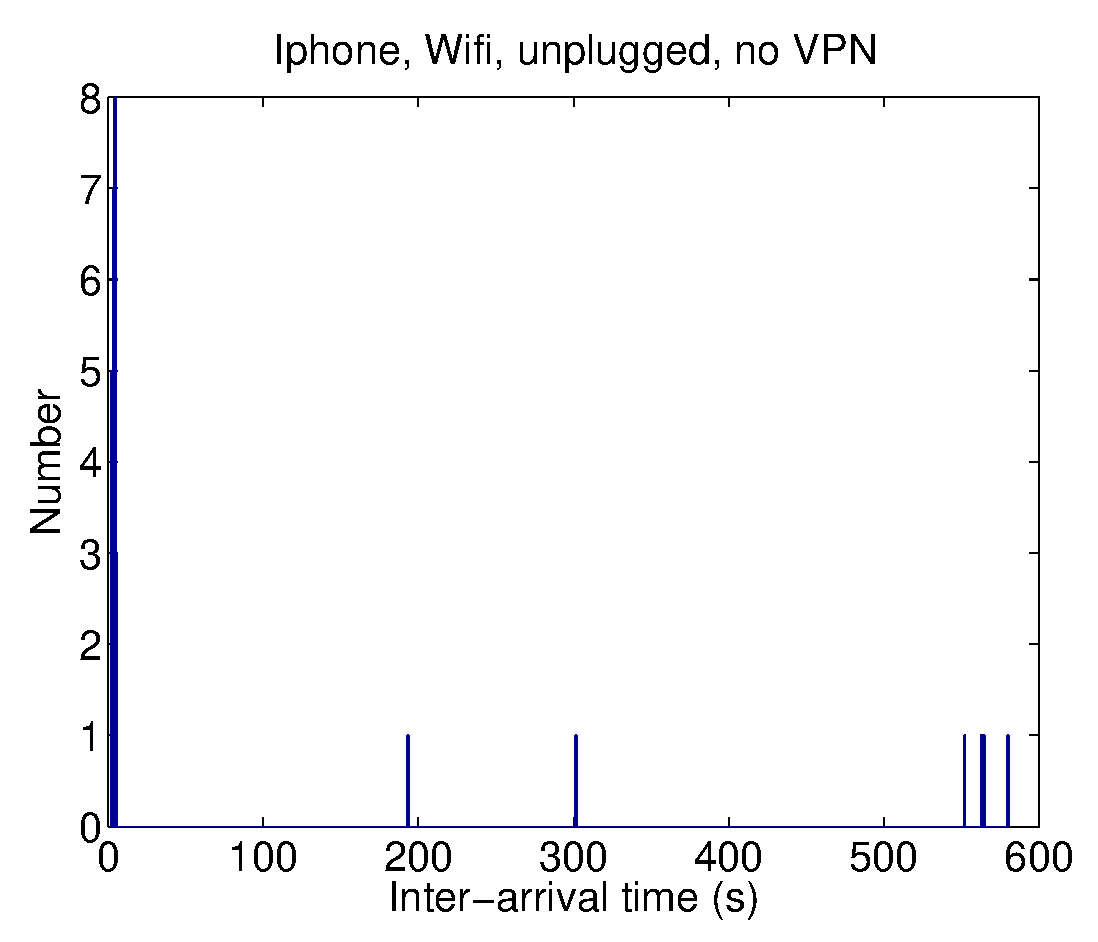
\includegraphics[width=0.8\linewidth]{../../code/pushNotification/Fig/bw_iphone_wifi_unplug_novpn_interTs.eps}
%  \caption{Distribution of the interarrival times of Ethernet frames
%    for a one hour experiment with an idle \iphone{} unplugged, with \wifi{} 
%    enabled, and no VPN enabled. For each bin of 1 second, we count
%    the number of interarrivals in that bin.}
%  \label{fig:push_w_interTs}
%\end{figure}


Surprisingly, even though the \iphone{} is idle, the traffic pattern
is not regular (Fig.~\ref{fig:push_w3_ts}). To
understand this irregularity, we made a new experiment with cellular
disabled. The largest
interarrival is still in the order of 550 seconds, as in the case with
cellular enabled, but we have less variety in the interarrival times. This
is confirmed by Fig.~\ref{fig:push_w_ts} that shows a regular
succession of short periods during which frames are exchanged and long
periods during which the wifi interface is not associated to the
access point.



Therefore, there is an evidence that the cellular connection triggers
the association of the \iphone{} \wifi interface with the access
point. This is confirmed by experiments we performed with iMessage, 
which uses the push notification infrastructure of Apple. When both
cellular and \wifi{} are enabled on an \iphone{}, a permanent connection to
the push notification infrastructure of Apple is setup on the cellular
interface. Each time an iMessage is received, it is piggybacked on the
push notification message (when short enough). Interestingly, the \wifi{}
interface is always woken-up even if no payload is sent on it. We
don't know the exact reason for this behavior, but it may have an
adverse impact of battery life for users with frequent push
notifications, \eg, heavy users of SMS, twitter, facebook, games, \etc



\begin{figure}
\centering
        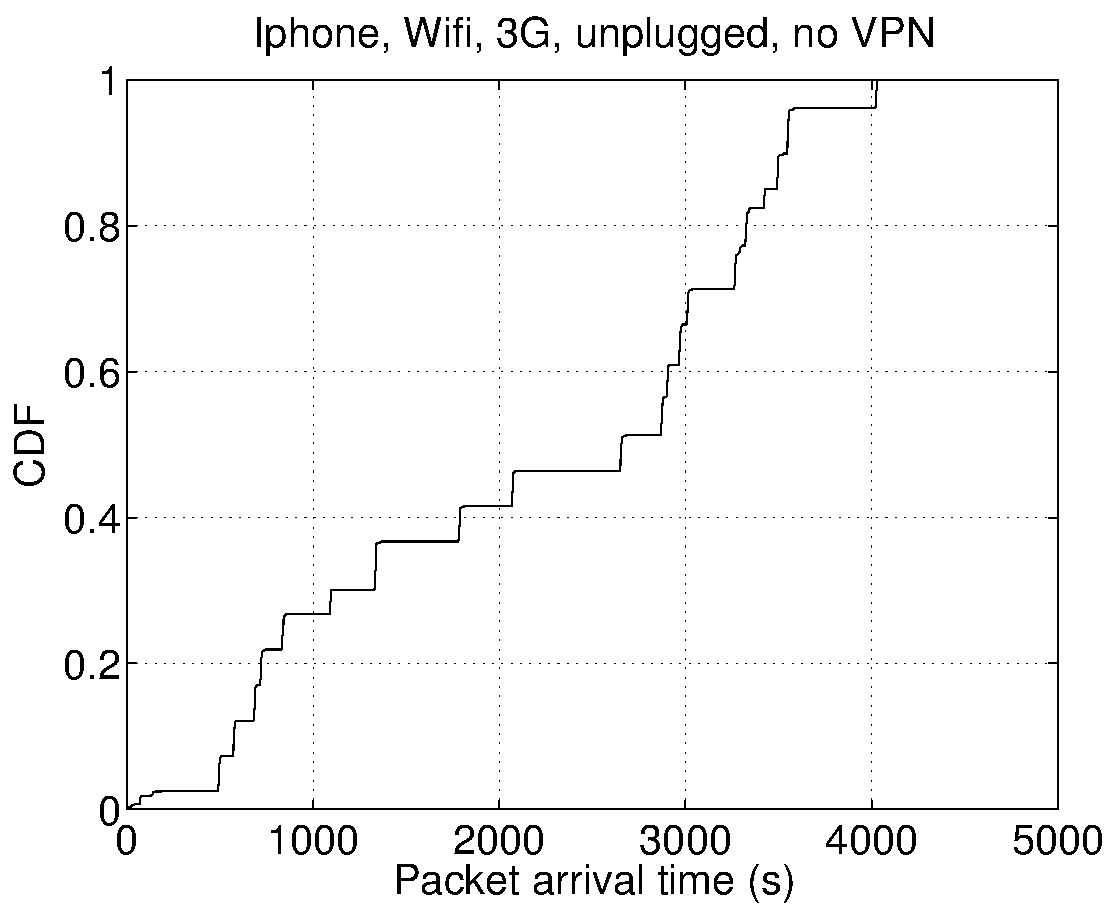
\includegraphics[width=0.8\linewidth]{../../code/pushNotification/Fig/bw_iphone_wifi_3g_unplug_novpn_ts.pdf}
  \caption{Cumulative distribution of the Ethernet frames
          arrival with time for a one hour experiment with an idle
          \iphone{} unplugged, with \wifi{} and cellular enabled, and no VPN
          enabled.}
  \label{fig:push_w3_ts}
   \vspace{\postfigspace}
\end{figure}


In summary, APNS allows apps to interact with the user despite a strict energy-saving policy that 
prevents apps running in the background; however, \emph{the systematic wake up of
the wifi interface might lead to an unnecessary severe increase in power
consumption}. 


\begin{figure}
\centering
        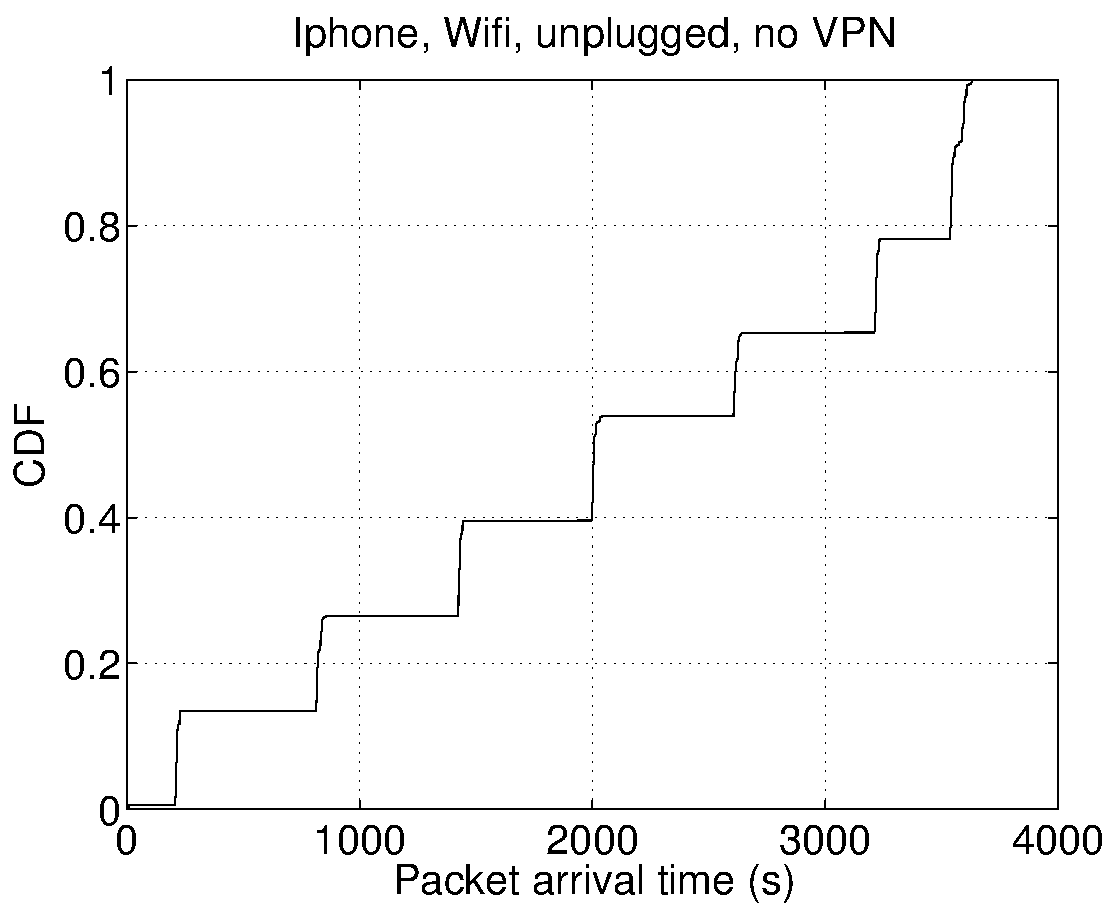
\includegraphics[width=0.8\linewidth]{../../code/pushNotification/Fig/bw_iphone_wifi_unplug_novpn_ts.pdf}
  \caption{Cumulative distribution of the Ethernet frames
          arrival with time for a one hour experiment with an idle
          \iphone{} unplugged, with \wifi{} enabled, and no VPN
          enabled.}
  \label{fig:push_w_ts}
   \vspace{\postfigspace}
\end{figure}

%We observed this same behavior on the tcpdump traces used to plot
%Fig.~\ref{fig:push_w3_ts}. We observe that the \wifi{} interface is
%woken-up (we observe a specific ARP and DHCP exchange that takes place
%for each \wifi{} association to the access point), but no payload is
%exchanged. In this case, as we do not use a VPN, we cannot monitor the
%3G traffic using \meddle{}, but we guess that traffic received on the
%3G interface trigger the wake of the \wifi{} interface. We plan to
%further explore this issue. 

%\begin{figure}
%\centering
%        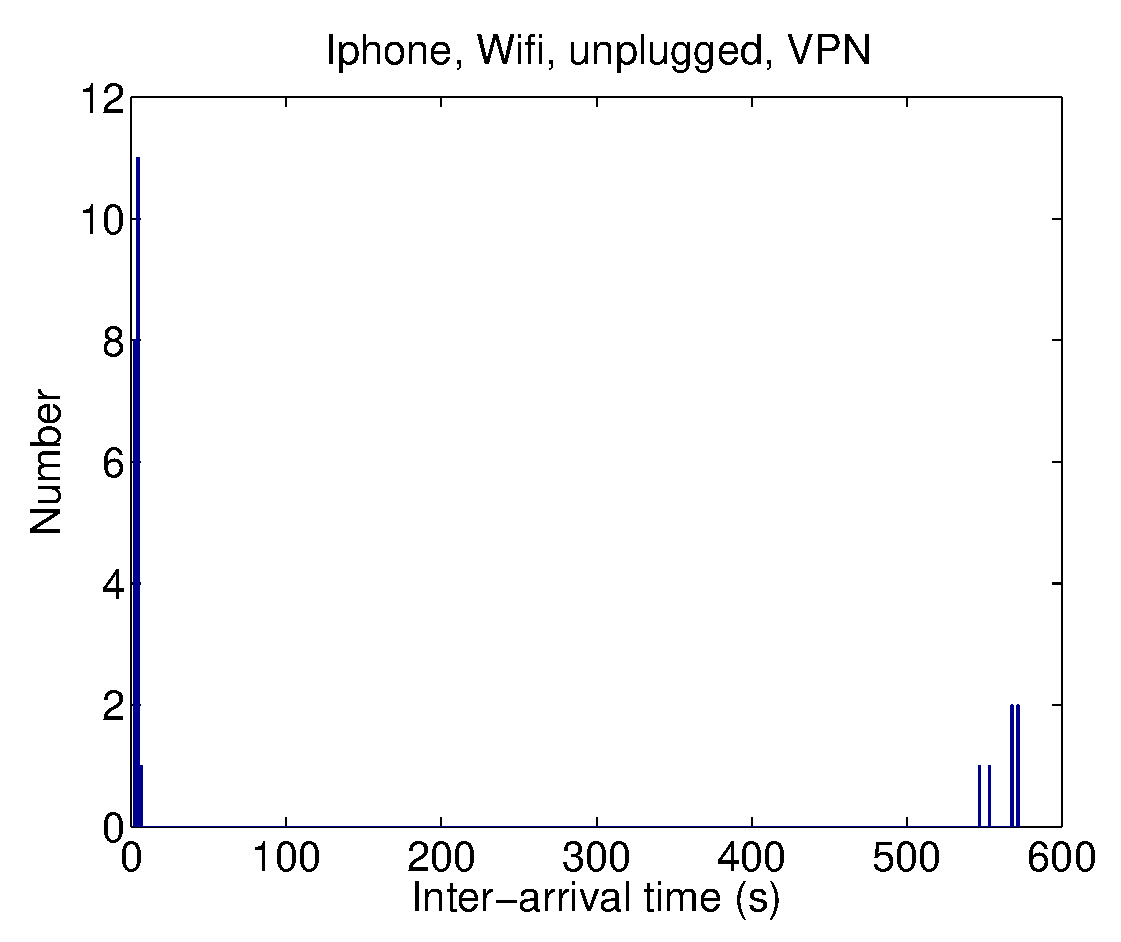
\includegraphics[width=0.8\linewidth]{../../code/pushNotification/Fig/bw_iphone_wifi_unplug_vpn_interTs.eps}
%  \caption{Distribution of the interarrival times of Ethernet frames
%    for a one hour experiment with an idle \iphone{} unplugged, with \wifi{}
%    enabled, and VPN enabled. For each bin of 1 second, we count
%    the number of interarrivals in that bin.}
%  \label{fig:push_wv_interTs}
%\end{figure}




\noindent\emph{Behavior when \meddle is enabled.} We performed a third set of experiments with the VPN enabled. This set
of experiments shows the interaction between \meddle 
and the power management policy. We see in
%Fig.~\ref{fig:push_wv_interTs} and 
Fig.~\ref{fig:push_wv_ts} that
there is no noticeable differences when enabling \meddle with \wifi{} only. However,
when enabling both \wifi and cellular the frames interarrival time
%(Fig.~\ref{fig:push_w3v_interTs}) 
and the cumulative arrival of frames (Fig.~\ref{fig:push_w3v_ts}) is
significantly different. This difference between scenarios with and
without cellular is due to the persistence of the cellular connection. Indeed, on
the one hand, if messages are sent to the device when the cellular connection is disabled,
they will be lost if the \wifi interface is sleeping. Therefore, the
\wifi association periods are triggered by an internal device policy
only. On the other hand, when the cellular connection is enabled, all
messages sent to the device will be received. If the \wifi interface
is sleeping, messages received on the cellular interface will wake up the
\wifi interface. In that case, the \wifi association periods are not
only triggered by an internal device policy, but by external events
too, which explains the very different interarrival times seen in
Fig.~\ref{fig:push_w3_ts} and Fig.~\ref{fig:push_w_ts}, and in
Fig.~\ref{fig:push_wv_ts} and Fig.~\ref{fig:push_w3v_ts}.


\begin{figure}
\centering
        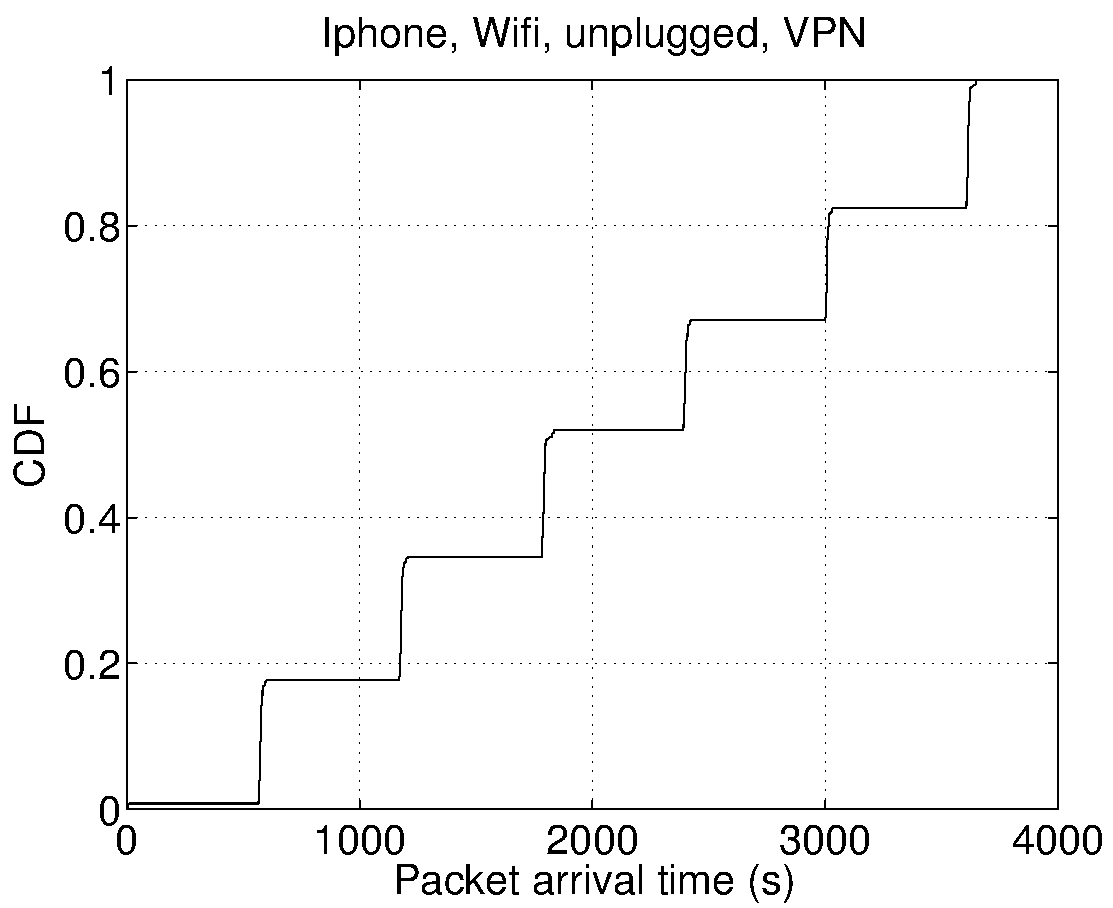
\includegraphics[width=0.8\linewidth]{../../code/pushNotification/Fig/bw_iphone_wifi_unplug_vpn_ts.pdf}
  \caption{Cumulative distribution of the Ethernet frames
          arrival with time for a one hour experiment with an idle
          \iphone{} unplugged, with \wifi{} enabled, and VPN
          enabled.}
  \label{fig:push_wv_ts}
   \vspace{\postfigspace}
\end{figure}


The main question that remains is: what are these messages received on
the cellular interface? In Fig.~\ref{fig:push_w3v_ts}, we observe a pattern
with a periodicity of around 45 seconds. This pattern does not exist
when the VPN is disabled as shown in Fig.~\ref{fig:push_w3_ts}. We
conclude that this periodicity is mostly due to keep alive messages of the
VPN for NAT traversal. In Fig.~\ref{fig:push_w3_ts}, we observe what looks like
a random wake up of the \wifi interface when the VPN is disabled. We
explored tcpdump traces for this scenario and for the scenario with
the VPN enabled, looking for messages that explain the apparent
randomness, but we did not find any such messages. Therefore, we guess
that packets that do not use the VPN tunnel are received on the cellular 
interface. Such packets might be sent by the cellular provider to the
device. 

 
% \tbd{It will probably be too short for the deadline, but I need to see
% on the meddle logs what are these 3G messages. I cannot get them from
% my setup. I guess that the VPN is using keep alive message every 45
% seconds. As the 3G connection never sleep, receiving such a packet
% trigger the wake-up of the \wifi{} interface. When 3G is disabled, the
% keep alive messages cannot prevent the \wifi{} interface to
% sleep. Ashwin, if you are aware of such a timer in your VPN config, we
% can safely state my guess in the paper.}

In conclusion, though \meddle appears to capture all IP traffic it may
miss traffic in the circuit switched network when a cellular connection is enabled.

\begin{figure}
\centering
        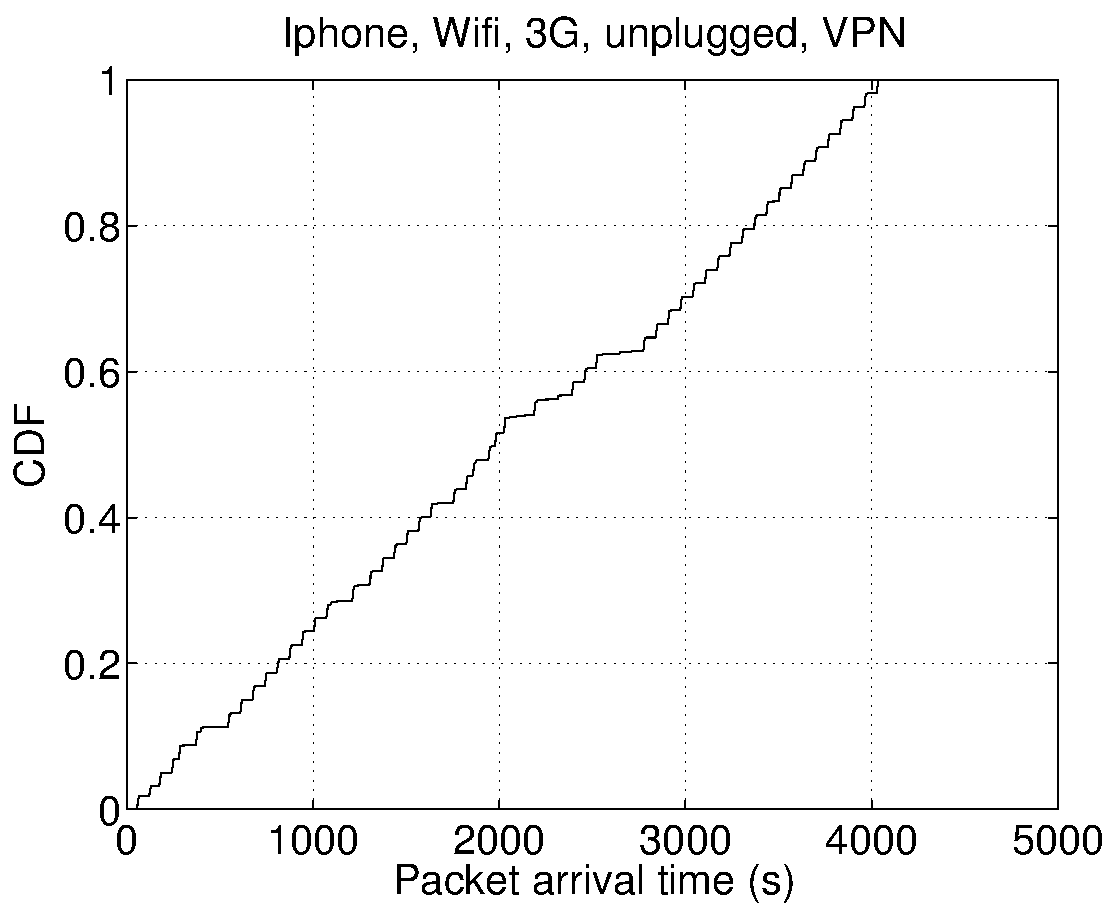
\includegraphics[width=0.8\linewidth]{../../code/pushNotification/Fig/bw_iphone_wifi_3g_unplug_vpn_ts.pdf}
  \caption{Cumulative distribution of the Ethernet frames
          arrival with time for a one hour experiment with an idle
          \iphone{} unplugged, with \wifi{} and cellular enabled, and VPN
          enabled.}
  \label{fig:push_w3v_ts}
   \vspace{\postfigspace}
\end{figure}


\subsection{Case Study: Longitudinal Measurements }
\label{sec:case-study-google}



% 1353489965.972204       7S1qUBBGGUg     24.19.59.238    45867   173.194.79.138  80      1       GET     suggestqueries.google.com       /complete/search?hl=en&ds=yt&client=androidyt&hjson=t&oe=UTF-8&q=a      -       Apache-HttpClient/UNAVAILABLE (java 1.4)        0       356     200     OK      -       -       -       (empty) -       -       -       -       -       application/json; charset=UTF-8 chunked text/plain      -       -
% 1353489966.199133       7S1qUBBGGUg     24.19.59.238    45867   173.194.79.138  80      2       GET     suggestqueries.google.com       /complete/search?hl=en&ds=yt&client=androidyt&hjson=t&oe=UTF-8&q=aw     -       Apache-HttpClient/UNAVAILABLE (java 1.4)        0       321     200     OK      -       -       -       (empty) -       -       -       -       -       application/json; charset=UTF-8 chunked text/plain      -       -
% 1353489966.471227       7S1qUBBGGUg     24.19.59.238    45867   173.194.79.138  80      3       GET     suggestqueries.google.com       /complete/search?hl=en&ds=yt&client=androidyt&hjson=t&oe=UTF-8&q=awe    -       Apache-HttpClient/UNAVAILABLE (java 1.4)        0       300     200     OK      -       -       -       (empty) -       -       -       -       -       application/json; charset=UTF-8 chunked text/plain      -       -
% 1353489966.881255       7S1qUBBGGUg     24.19.59.238    45867   173.194.79.138  80      4       GET     suggestqueries.google.com       /complete/search?hl=en&ds=yt&client=androidyt&hjson=t&oe=UTF-8&q=awes   -       Apache-HttpClient/UNAVAILABLE (java 1.4)        0       301     200     OK      -       -       -       (empty) -       -       -       -       -       application/json; charset=UTF-8 chunked text/plain      -       -
% 1353489967.365324       7S1qUBBGGUg     24.19.59.238    45867   173.194.79.138  80      5       GET     suggestqueries.google.com       /complete/search?hl=en&ds=yt&client=androidyt&hjson=t&oe=UTF-8&q=aweso  -       Apache-HttpClient/UNAVAILABLE (java 1.4)        0       302     200     OK      -       -       -       (empty) -       -       -       -       -       application/json; charset=UTF-8 chunked text/plain      -       -
% 1353489968.001541       7S1qUBBGGUg     24.19.59.238    45867   173.194.79.138  80      6       GET     suggestqueries.google.com       /complete/search?hl=en&ds=yt&client=androidyt&hjson=t&oe=UTF-8&q=awesom -       Apache-HttpClient/UNAVAILABLE (java 1.4)        0       303     200     OK      -       -       -       (empty) -       -       -       -       -       application/json; charset=UTF-8 chunked text/plain      -       -
% 1353489968.303481       7S1qUBBGGUg     24.19.59.238    45867   173.194.79.138  80      7       GET     suggestqueries.google.com       /complete/search?hl=en&ds=yt&client=androidyt&hjson=t&oe=UTF-8&q=awesome        -       Apache-HttpClient/UNAVAILABLE (java 1.4)        0       304     200     OK      -       -       -       (empty) -       -       -       -       -       application/json; charset=UTF-8 chunked text/plain      -       -
% 1353489968.469449       7S1qUBBGGUg     24.19.59.238    45867   173.194.79.138  80      8       GET     suggestqueries.google.com       /complete/search?hl=en&ds=yt&client=androidyt&hjson=t&oe=UTF-8&q=awesome+       -       Apache-HttpClient/UNAVAILABLE (java 1.4)        0       330     200     OK      -       -       -       (empty) -       -       -       -       -       application/json; charset=UTF-8 chunked text/plain      -       -
% 1353489969.221635       7S1qUBBGGUg     24.19.59.238    45867   173.194.79.138  80      9       GET     suggestqueries.google.com       /complete/search?hl=en&ds=yt&client=androidyt&hjson=t&oe=UTF-8&q=awesome+t      -       Apache-HttpClient/UNAVAILABLE (java 1.4)        0       345     200     OK      -       -       -       (empty) -       -       -       -       -       application/json; charset=UTF-8 chunked text/plain      -       -
% 1353489969.551634       7S1qUBBGGUg     24.19.59.238    45867   173.194.79.138  80      10      GET     suggestqueries.google.com       /complete/search?hl=en&ds=yt&client=androidyt&hjson=t&oe=UTF-8&q=awesome+to     -       Apache-HttpClient/UNAVAILABLE (java 1.4)        0       390     200     OK      -       -       -       (empty) -       -       -       -       -       application/json; charset=UTF-8 chunked text/plain      -       -
% 1353489969.953698       7S1qUBBGGUg     24.19.59.238    45867   173.194.79.138  80      11      GET     suggestqueries.google.com       /complete/search?hl=en&ds=yt&client=androidyt&hjson=t&oe=UTF-8&q=awesome+to+    -       Apache-HttpClient/UNAVAILABLE (java 1.4)        0       383     200     OK      -       -       -       (empty) -       -       -       -       -       application/json; charset=UTF-8 chunked text/plain      -       -


%\begin{table}
%\begin{center}
%\begin{tabular}{|c|c|l|}
%\hline
%Time & Bytes & Query \tabularnewline
% & Downloaded & String\tabularnewline
%\hline 
%1353489965.97 & 356 & a \tabularnewline
%\hline
%1353489966.19& 321 & aw\tabularnewline
%\hline
%1353489966.47& 300 & awe\tabularnewline
%\hline
%1353489966.88& 301 & awes\tabularnewline
%\hline
%1353489967.36& 302 & aweso\tabularnewline
%\hline
%\end{tabular}
%\end{center}
%\caption{Table}
%\label{tab:ExampleGoogleSearch}
%\end{table}
A key advantage of our approach is that we can monitor app behavior 
over time and as updates occur. This can lead to surprising or otherwise 
unpublicized revelations about network activity.

One prominent example is Google searches from mobile devices. In the 
desktop environment, we have grown accustomed to these searches 
occurring over HTTPS connections, which protects user privacy, \eg, from 
carriers and from other users at open \wifi hotspots. 

In the mobile environment, however, we noticed that the default 
browsers on iOS and Android send user queries in the clear. In fact, 
each letter is sent as the user types it for the purpose of Google Suggestions. 
We
observed this behavior on Android 4.0 and Android 4.1. In the case of iOS devices we observed search queries
in the clear on devices running iOS 5. 

Interestingly, as of iOS 6 and Android 4.2 these searches are now sent using HTTPS, addressing 
a significant privacy vulnerability. To the best of our knowledge this 
change has not been publicized. 

%We now use Google search as an example of longitudinal studies that
%are possible using using Meddle.
%
%In \fref{tab:ExampleGoogleSearch} we present a sample search session on
%Android 4.0. During this sesssion, we observe that each key stroke by
%the user resulted in a unique GET query made to a Google server. We
%observe similar behavior on Android 4.0, Android 4.1, and Android 4.2
%\tbd{confirm}. In the case of iOS devices we observed search queries
%in the clear on devices running iOS 5. On devices running iOS 6 we
%observe that search queries take place over SSL. \tbd{Privacy similar
%  to desktop sentence.}


%\subsection{Case Study: Misbehaving Apps}
%\label{sec:case-study-filtering}
\subsection{Case Study: Misbehaving Apps}
\label{sec:case-study-filtering}

    Smartphone users are often faced with the decision whether or not to trust an app downloaded from the iPhone App Store or the Android Market.
    The user can access some information \emph{a priori} regarding the app's behavior, \eg{} via reading reviews or inspecting the permissions requested, but this provides at best an incomplete and at worst and incorrect view.
    Although some undesirable app behavior is obvious -- \eg{} pushing advertisements to the notifications bar, installing unwanted third-party software, \etc{} -- the app's network behavior remains generally invisible to the user even after installation. \meddle allows users and researchers to see this behavior and draw conclusions about whether it is appropriate. 
     To guide our analysis in the rest of this section, we define several key network-usage properties that describe a ``well behaved'' app:
    \begin{itemize}
        \item Protection of personally identifiable information (PII): transmitting PII only when required for application functionality, and if transmitting PII, doing so over HTTPS rather than HTTP.
        \item Conservation of power and data quota by making only necessary use of network.
        \item Communication only with servers needed for the applications intended purpose, with preferably a limited number of entities contacted by the app overall.
    \end{itemize}

\noindent\textbf{Survey of privacy violations in the wild.} In our dataset, we were surprised to find several examples of PII sent in the clear. Specifically, we searched for IMEI (device unique identifiers) and 
GPS coordinates in HTTP request strings. Offending apps include The New York Times, The Weather Channel, Fox News, ESPNCricInfo, FirstPost and 
Angry Birds. For many of these apps, the privacy violations are due to included software for displaying ads. The key takeaway is that privacy 
violations from tracking software is pervasive and often easy to detect. When using \meddle, users limit their exposure to eavesdroppers 
because the connection to the \meddle server is encrypted. Further, in the next section we discuss how \meddle can strip this information. 
  
\noindent\textbf{Controlled experiments} While the above examples indicate clear examples of undesirable app behavior, 
it is more difficult to determine which traffic is strictly necessary for app functionality and which can be removed through blocking 
at a \meddle server. 
    With this in mind, we used \meddle to perform a short app-by-app analysis of network usage behavior.
    
       We downloaded five of the most popular apps from the Android Market and installed them on an fresh install of Android 4.1.
       The apps fall into the following categories: two popular games,a weather app, a settings 
        management app, and a risqu\'{e} app serving various images. We interacted with each app for between 7 and 15 minutes 
        to understand network behavior when the app is being used.

    \noindent{\bf Leaking PII.}
    None of the apps we installed for these experiments leaked PII over HTTP. However, there was evidence that the weather app was making use of a tracking service, contacting an third-party service which markets itself as specializing in `device tracking and fraud prevention.'
    It is unclear why a weather app requires a service for fraud prevention.

    \noindent{\bf Third Party Contacts.} 
    The settings app and the game apps contacted a limited number of third parties.
    The settings app contacted Amazon, Google, a hosting service, and two CDN services.
    One game app contacted only Amazon, Google, and a single CDN provider, the other contacted only Amazon, Google, a private server belonging to the game developer, and three CDN/Ad services.
    The weather app and the risqu\'{e} app both contacted a large number of third party services; the weather app contacted 10 and the risqu\'{e} app contacted 19. 

   \noindent{\bf Resource Consumption.}
   Finally, we considered resource consumption towards both battery life and data caps.
    The risqu\'{e} app by far made the most impact towards data cap consumption: on average, it consumed 23.37 Kb per second of use.
    This is not entirely surprising, given that the app was serving images, but this figure is magnified by the fact that the app downloaded and installed several additional (unrequested) apps to the phone.
    The weather app and settings app consumed 4.49 Kbps and 6.27 Kbps respectively; the games apps had much more limited bandwidth consumption with only 1.5 and 1.7 Kbps consumed each.

    To evaluate behavior towards battery life, we considered the fraction of 30-second intervals during which no traffic was sent by the phone, rather than the amount of traffic sent overall. 
    We require this different metric because, \eg{} small amounts of traffic, sent frequently leave the radio on for an extended period of time, thus bandwidth is not the best indicator of radio use.
    The games apps, which were the best performers in terms of bandwidth consumption, were some of the worst performers in terms of radio usage: 78\% and 66\% of 30-second intervals generated network traffic.
    However, the worst performer overall was the settings app, which generated traffic during 85\% of 30-second intervals.
    The weather app, and the risqu\'{e} app generated traffic during 23\% and 49\% of 30-second intervals respectively.

    \noindent{\bf Summary.}
    The risqu\'{e} app acted maliciously in installing unwanted apps; whether or not the weather app acted maliciously through its use of a third party tracking service is unclear.
    However, all apps, even those that were decidedly non-malicious, had some network behavior worth some concern by contacting multiple third parties and making inneficient use of bandwidth and battery life.
    \meddle can help ameliorate some of these concerns: data consumption and third-party contacts can be restricted by blocking DNS lookups and connections to ad services. 
    In \S\ref{sec:filtering}, we discuss these filtering capabilities further.



\subsection{Case Study: Traffic Optimization}
\label{sec:case-study-compression}

In our data set we observed that 42.45\% of the all the HTTP flows (1.06\% by volume) have 
a mime-type of ``text.'' This implies that the content can be potentially compressed by the 
remote server. We observe that 38\% of such flows (3.42\% by volume) are, in fact, compressed. 
Importantly, our analysis reveals that 23\% of HTTP flows are uncompressed, and these flows 
contribute only 0.5\% of our users' total data. Thus, we believe there are few meaningful 
opportunities for injecting compression at a meddlebox; instead, we believe most improvements 
will come from transcoding media content to lower bitrates and resolution. 

Interestingly, we also observe that compression is counter-productive for 4\% of 
the all the flows that have a mime-type of "text" -- the volume of data after 
compression is larger than the volume before compression. In Table~\ref{tab:compression} we present the top five  
sources of traffic for which compression is counterproductive. As one example, we find 
that despite good intentions, Google's use of compression for search responses generally 
does more harm than good.

\begin{table}
\begin{center}
\begin{tabular}{|l|l|}
\hline
\textbf{Android} & \textbf{iOS} \tabularnewline
\hline
mercuryapps.foxnews.com & www.engadget.com \tabularnewline
\hline
www.google.com & itunes.apple.com \tabularnewline
\hline
www.quora.com & iadctest.qwapi.com \tabularnewline
\hline
opml.radiotime.com & www.google.com \tabularnewline
\hline
www.pandora.com & beacon.flipboard.com  \tabularnewline
\hline
\end{tabular}
\caption{Top five sites using counterproductive compression.}
\label{tab:compression}
\end{center}
\vspace{-1.5em}
\end{table}








 




%%% Local Variables: 
%%% mode: latex
%%% TeX-master: "main"
%%% End: 
